\section{Background}\label{sec:background}

% This section introduces \paxos and RDMA background.

\subsection{\paxos}\label{sec:paxos}
% \paxos background. Keys:
% Leader, backup.
% Persistent storage. 
% Network round trips in normal case. Latency.
\paxos~\cite{paxos:complex,paxos,paxos:simple,paxos:live,paxos:fast,
paxos:practical} runs the same program and its data on a group of replicas 
and enforces a strongly consistent order of inputs across replicas. Because 
a consensus can be achieved as long as a majority of replicas agree, \paxos is 
well known for tolerating various faults, including minor replica failures 
and packet losses. If the leader replica fails, \paxos elects a new leader from 
the backups.

To handle replica failovers, standard \paxos must log inputs in local 
stable storage. When a new input comes, the \paxos leader writes this input in 
local stable storage. The leader then starts a new consensus round among 
replicas. A backup also writes the received consensus request in local storage 
if it agrees on this request. Since logging is done by each replica locally, it 
is scalable.

% The second feature is safety. As long as a quorum (typically, majority) of 
% replicas agree on this input (\ie, this input is \emph{committed}), \paxos 
% guarantees that all replicas consistently agree to process this input. If a 
% replica sees that an input consensus has been reached, this consensus must have 
% really been reached by at least a majority of replicas. Safety ensures that if 
% a consensus has not really been reached, no replica will ``think" that this 
% consensus has been reached.

% Durability and safety make replicas consistently agree on each input and 
% tolerate various faults, including machine failures and network errors. As 
% consensus rounds move on, \paxos consistently enforces the same sequence of 
% inputs across replicas. It also enforces same execution states across replicas 
% without divergence if a program behaves as a deterministic state machine (\ie, 
% always produces the same output on the same input).

% Normal case, round trip.
The consensus latency of \paxos protocols is notoriously high and 
unscalable~\cite{zookeeper,scatter:sosp11}. As datacenters incorporate 
faster networking hardware and more CPU cores, traditional \paxos 
protocols~\cite{libpaxos,spaxos:srds12,crane:sosp15,rex:eurosys14,zookeeper} are 
having fewer performance bottlenecks on network bandwidth and CPU resources. 

% Arrakis~\cite{arrakis:osdi14} reported that a \v{ping} program spent over 70\% 
% latency in these two layers.

However, software TCP/IP layers and OS kernels remain performance 
bottleneck~\cite{arrakis:osdi14}. To quantify this bottleneck, we evaluated 
four traditional consensus protocols on 24-core computers with 40Gbps 
network, and we spawned 24 concurrent consensus clients. When changing the 
replica group size from three to nine, although network and CPUs were not 
saturate, the consensus latency of three protocols drastically increased by 
\tradlatencyincreaselow to \tradlatencyincreasehigh 
(Figure~\ref{fig:scalability}), and \systemcostlow to \systemcosthigh of this 
increase was in OS kernel. If only one consensus client was spawned, the latency 
increase on the number of replicas was more gentle 
(Table~\ref{tab:traditional-latency}).

This evaluation also shows that both the number of concurrent requests and 
replicas make \paxos latency increase drastically. This problem becomes worse 
as server programs tend to support more concurrent requests and advanced SMR 
systems such as Azure deploy seven to nine replicas~\cite{azure:book} 
(for upgrades of multiple replicas).
% Therefore, existing 
% systems (\eg, Scatter) deploy less than one dozen replicas in each \paxos group.


% For instance, in an 
% efficient, practical 
% \paxos implementation~\cite{paxos:practical}, each input in normal case takes 
% one consensus round-trip between every two replicas (one request from the leader 
% and one reply from a backup).


\subsection{RDMA}\label{sec:rdma}
% Queue Pair. Completion Queue.
% Fastest: RDMA one-sided write. % Define one-side RDMA write as WRITE.
% UC and RC.
% RC Need an ACK. But can also do selective signaling.
RDMA architectures (\eg, Infiniband~\cite{infiniband} and RoCE~\cite{roce})
become common within a datacenter due to its ultra low latency, high 
throughput, and its decreasing prices. The ultra low latency of RDMA not only 
comes from its kernel bypassing feature, but also its dedicated network stack 
implemented in hardware. Therefore, RDMA is considered the fastest kernel 
bypassing 
technique~\cite{herd:sigcomm14,pilaf:usenix14,dare:hpdc15}; it is several times 
faster than software-only kernel bypassing techniques (\eg, DPDK~\cite{dpdk} 
and Arrakis~\cite{arrakis:osdi14}).

RDMA has three operation types, from fast to slow: one-sided 
read/write operations, two sided send/recv operations, and IPoIB (IP over 
Infiniband). IPoIB can run unmodified socket programs, but it is several times 
slower than the other two primitives. A one-sided RDMA write 
operation can directly write from one replica's memory to a remote 
replica's memory without involving the remote OS kernel or CPU. Prior 
work~\cite{pilaf:usenix14} shows that one-sided operations are up to 2x faster 
than two-sided operations~\cite{fasst:osdi16}, so \xxx uses one-sided operations 
(or ``WRITE" in this paper). On a WRITE succeeds, the remote NIC sends
an RDMA ACK to local NIC.

A one-sided RDMA communication between a local and a remote NIC needs
a Queue Pair (QP), including a send queue and a receive 
queue. Each QP has a Completion Queue (CQ) to store ACKs. A QP 
belongs to a type of ``XY": X can be R (reliable) or U (unreliable), and Y can 
be C (connected) or U (unconnected). HERD~\cite{herd:sigcomm14} shows 
that WRITEs on RC and UC OPs incur almost same latency, so \xxx 
uses RC QPs.

% \xxx's implementations mainly use RC QPs, because such a reliable, connected QP 
% guarantees in-order, non-corrupted delivery in normal case. However, RC QPs may 
% still lose packets in typical \paxos exceptional cases (\eg, hardware failures, 
% OS crashes, or server program restarts).



Normally, to ensure a WRITE resides in remote memory, the local replica 
normally busily polls an ACK from the CQ before it proceeds 
(or \emph{signaling}). Polling ACK is time consuming as it involves 
synchronization between the NICs on both sides of a CQ. We looked into the ACK 
pollings in a fastest RDMA-based \paxos protocol \dare~\cite{dare:hpdc15}, and 
we found that, although \dare is highly optimized (its leader maintains one 
global CQ to receive all backups' ACKs in batches), polling ACKs is still time 
consuming: when the CQ was empty, it took 0.039$\sim$0.12 \us; when the CQ has 
one or more ACKs, it took 0.051$\sim$0.42 \us.
% Therefore, \xxx 
% avoids ACKs.

% As the number of ACKs is linear 
% to both the number of concurent requests and replicas, polling ACKs becomes one 
% major scalability bottleneck in \dare (\S\ref{sec:evaluation}).

% If the 
% number of polling ACK operations is linear to the replica group size, a \paxos 
% protocol will incur scalability bottlenecks when the size is large 
% (\S\ref{sec:evaluation}).

Fortunately, depending on protocol logic, one can do \emph{selective 
signaling}~\cite{herd:sigcomm14}: it only checks for an ACK after pushing a 
number of WRITEs. Because \xxx's protocol logic does not rely on RDMA ACKs, 
it just occasionally invokes selective signaling to clean up ACKs.

% To 
% perform RDMA operations, the process and the remote process establishes a 
% communication end point called Queue Pairs (QP). The remote memory access is 
% fully operated by hardware without involing software network layers, OS kernel, 
% or CPU of the remote machine. QP are lossless in normal case, but packet losses 
% may happen during machine or software (\eg, the server program) restarts.

% One-side RDMA operations can totally write from one machine's memory to a 
% remote machine's memory directly. However, for one-sided operations, the remote 
% machine's memory is not aware of the write either, so a careful protocol design 
% is necessary when one-sided operations are used.

\section{\xxx Overview}\label{sec:overview}

% This section first presents \xxx's architecture, including its 
% deployment model and key components (\S\ref{sec:arch}).
 
% \subsection{Architecture}\label{sec:arch}



% \begin{figure*}[!htb]
% \centering
% 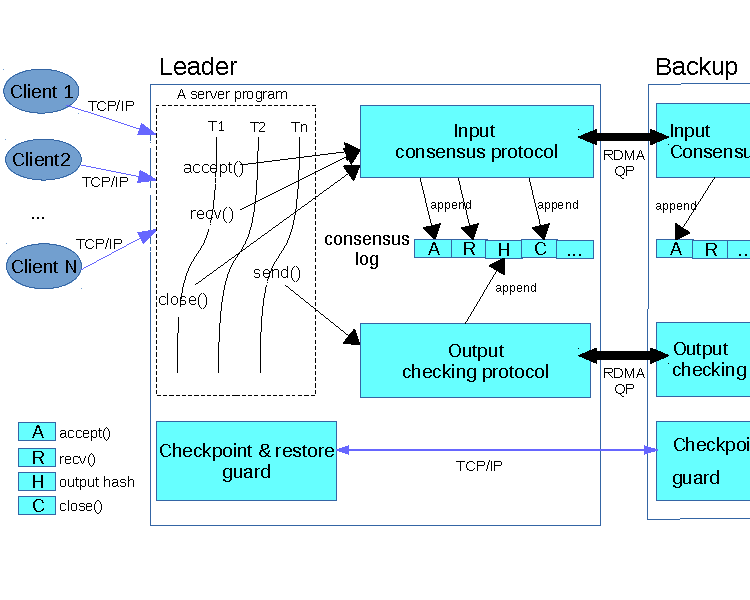
\includegraphics[width=0.5\textwidth]{figures/arch}
% \vspace{-.10in}
% \caption{{\em The \xxx Architecture.} \rm {\xxx components are shaded (and in
%   green).}} \label{fig:arch}
% \vspace{-.05in}
% \end{figure*}

% TBD. Input coordinator and output checker. Components.

% System model. Replicas. RDMA. LAN. Clients.
\xxx follows a typical SMR deployment scenario: it runs replicas of a server 
program in a datacenter. Replicas 
connect with each other using RDMA QPs. Client programs located in LAN or WAN. 
The \xxx leader handles client requests and runs its RDMA-based 
protocol to coordinate inputs across replicas.
% If a backup receives client 
% requests, it deny the requests and reply the leader's IP.

% \xxx intercepts four types of 
% socket operations: the \accept type, the \recv type, the \send type, and the 
% \close type. 
Figure~\ref{fig:arch} shows \xxx's architecture. \xxx intercepts a server 
program's inbound socket calls (\eg, \recv) using a Linux technique called 
LD\_PRELOAD. \xxx involves four key components: a \paxos consensus protocol for 
input coordination (in short, the \emph{coordinator}), an output checking 
protocol (the \emph{checker}), a circular in-memory consensus log (the 
\emph{log}), and a guard process that handles checkpointing and recovering a 
server's process state and file system state (the \emph{guard}).

\begin{figure}[t]
\centering
\vspace{-.15in}
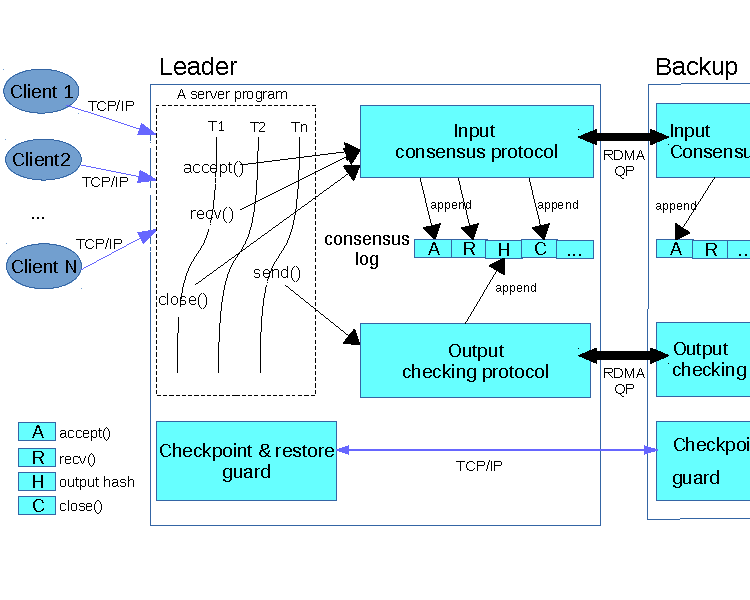
\includegraphics[width=.48\textwidth]{figures/arch}
\vspace{-.30in}
\caption{\em \xxx Architecture (key components are in
  blue).}
\vspace{-.2in}
  \label{fig:arch}
\end{figure}


% Coordinator: leader side. 
The coordinator is invoked when a server program thread calls an inbound socket 
call to manage a client socket connection (\eg, \accept and \close) or to 
receive inputs from the connection (\eg, \recv). On the leader side, \xxx 
executes the actual Libc socket call, extracts the returned value or inputs of 
this call, stores it in local SSD, appends a log entry to its local consensus 
log, and then invokes the coordinator for a new consensus request on 
``executing this socket call".

The coordinator runs a consensus algorithm (\S\ref{sec:input}), which WRITEs 
the local entry to backups' remote logs in parallel and polls the local log 
entry to wait quorum. When a quorum is reached, the leader thread simply 
finishes intercepting this call and continues with its server execution. As 
the leader's server threads execute more calls, \xxx enforces the same 
consensus log and thus the same socket call sequence across replicas.

% In this request, in order tell the 
% backups what socket 
% calls they should execute, this request also carries the latest request 
% viewstamp that has reached consensus (\ie, the latest committed request).

% This coordinator invokes a consensus request by: (1) assigns this call a 
% monotonically increasing index (\ie, a viewstamp) in the log, (2) builds a 
% socket call struct (\S\ref{sec:input}), (3) store the struct to persistent 
% storage, (4) appends it to the log according to the index, and (5) writes this 
% struct to all remote backup replicas' log.

% Coordinator: backup side.
On each backup side, the coordinator uses a \xxx internal thread called 
\emph{follower} to poll its consensus log for new consensus requests. If the 
coordinator agrees the request, the follower stores the log entry in local SSD 
and then WRITEs a consensus reply to the remote leader's corresponding log 
entry. A backup does not need to intercept a server's socket calls because the 
follower will just follow the leader's consensus requests on executing what 
socket calls and then forward these calls to its local server program.

% To respond consensus requests rapidly, each 
% backup coordinator spawns a dedicated thread. This thread runs a busy loop to 
% pull consensus requests from the consensus log. This high-perfomance thread 
% runs in a spare dedicated CPU core and elinimates context switches, unlike 
% traditional TCP/IP that block threads socket calls to wait for requests.

% The backup 
% coordinator then forwards all the requests up to the latest committed socket 
% call to its local server process. 

% Consensus log. Same in both leader and backups.
% A consensus log appending operation is invoked whenever a leader's server 
% executes a socket call (except \send calls, handled by output checker). The 
% leader coordinator just appends socket calls to the log and backups follow 
% socket calls in this log.

% Output checker: leader side. % Output checker: backup side.
The output checker is occasionally invoked as the leader's server program 
executes outbound socket calls (\eg, \send). For every 1.5KB (MTU size) of 
accumulated outputs per connection, the checker unions the previous hash with 
current outputs and computes a new CRC64 hash. After a fixed number of hashes 
are generated, the checker then invokes consensus across replicas, which 
compares the hash at its global hash index on the leader side.

This output consensus is based on the input consensus algorithm 
(\S\ref{sec:input}) except that backups carry their hash at the same hash index 
back to the leader. For this particular output consensus, the leader first 
waits quorum. It then waits for a few \us in order to collect more remote 
hashes. It then compares remote hashes it has.

If a hash divergence is detected, the leader optionally invokes the local guard 
to forward a ``rollback" command to the diverged replica's guard. The diverged 
replica's guard then rolls back and restores the server program to a latest 
checkpoint before the last successful output check (\S\ref{sec:output}). The 
replica then restores and re-executes socket calls to catch up. As output 
hash generations are fast and an output consensus is invoked occasionally, we 
did not observe performance impact on the checker.

% Then, for every \emph{Tcheck} hash generations, the checker invokes a consensus 
% request on this hash value. This output consensus is the same as the 
% coordinator's input consensus except that backups' output checkers send ACKs 
% with their own hash values with the same index, whenever the hash values are 
% ready (some backups may run slowly). When a majority of hashes are back, the 
% leader's output checker compares these values and then makes an effort to roll 
% back divergent replicas to a previous checkpoint before the last matching hash. 


% Guard: leader side. % Guard: backup sides.
% Question: how does the backup replicas know the last matching hash? Through 
% committed viewstamp for the \send.
% The leader's guard accepts roll-back requests from the output checker and 
% forwards the requests to the corresponding guard on another, divergent repilca. 
% The divergent replca's guard then rolls back the server program to a previous 
% checkpoint before the last matching one, and then invokes the local input 
% coordinator to re-forward the requests in stable storage to the server. There 
% is no a second output hash comparisons between backups and leader until the 
% leader invokes a new output checking consensus request next time.


% \subsection{Example}\label{sec:example}
% 
% \begin{figure}[t]
% \centering
% \begin{minipage}{.5\textwidth}
% \lgrindfile{code/example.cpp.lineno}
% \end{minipage}
% \vspace{-.1in}
% \caption{{\em A server example.}} \label{fig:example}
% \vspace{-.20in}
% \end{figure}
% 
% \begin{figure}[t]
% \centering
% \begin{minipage}{.5\textwidth}
% \lgrindfile{code/client.cpp.lineno}
% \end{minipage}
% \vspace{-.1in}
% \caption{{\em A client example.}} \label{fig:client}
% \vspace{-.05in}
% \end{figure}

% TBD. A simple server with recv(), accept(), and send(). Must have a 
% concurrency bug in this toy program? Race on global var or heap?

% Describe the example code.
% Describe the example code. Describe a 'set' command from key-value store.
% Figure~\ref{fig:example} shows a simplified server code based on the \redis 
% key-value store, and Figure~\ref{fig:client} shows a client cocde. The server 
% accepts a new connection from a client, receives one input request, process the 
% request, and then sends a reply. Suppose the client sends a ``SET a b" request.

% Input coordination protocol.
% Once the client calls its \connect, the leader's server program calls the 
% \accept call intercepted by \xxx. The leader's input coordinator then invokes 
% consensus on building a new connection by writing a struct for \accept to 
% remote backups with RDMA. Once a majority of backups agree, the leader machine 
% returns from the \accept call and continues to run.

% When a client program calls its \send, leader's server traps into \xxx's \recv 
% function call, which a invokes consensus on this new input ``SET a b". If 
% a consensus is made by a majority of replicas, the leader directly returns from 
% \recv and processes the request, and each replica's dedicated thread sets up 
% a new connection to the local server because the \recv consensus request 
% notifies the backups that the last call, \accept, has reached consensus.


% Output checking protcol.
% Challenge: what if leader does more sends and replicas do fewer sends?
% When a request is processed and the server is about to send reply to the 
% client, \xxx traps into the \send call, computes historical hash value on 
% inputs when 4K bytes (MTU size). Since this request is short, no output check 
% will be invoked at this time. All backups return consensus reply to the leader 
% with their own hash values if this value is available on their replica. 
% Similarly, backups do the earlier socket call: the backups' follower forwards 
% ``SET a b" request to the local server program.

% TBD: explain why we do not need to intercept poll() function.

% TBD Question: must ask Cheng. The close logic is not clear. What do the 
% leaders and backups do for close()? Why do we have to need a NOP (if 
% backup thread does not close its connection to local server, it does not 
% matter, right)? 
% Finally, the leader's server program executes a \close call. Similarly, the 
% leader invokes consensus on this call, and the backups have this \close call in 
% their log so that they can close the 

% TBD: what is the interesting outcome of this program running with Falcon? 
% Replicating all inputs without modifications? Any chart figure/schedule? 
% Two points so far: automatically replicating all inputs without modification; 
% can tolerate one replica failure; the other two can still process requests.